\documentclass[12pt,fleqn]{article}
\usepackage[utf8]{inputenc}
\usepackage[ngerman]{babel}
\usepackage{setspace}
\usepackage{amsmath, amsfonts, amssymb, amsthm}
\usepackage{mathtools}
\usepackage{blindtext}
\usepackage{graphicx}
\usepackage[paper=a4paper,left=25mm,right=25mm,top=25mm,bottom=25mm]{geometry}
\newcommand\textbox[1]{\parbox{.333\textwidth}{#1}}
\usepackage{setspace}
\usepackage{siunitx}

\begin{document}
\noindent{Name: Xuan Anh Nguyen\hfill SS 2021\hfill \\Matriculation number: 6895536\hfill}
 
\hrulefill
\vspace*{10mm} 
 
\begin{center}
	\Huge Text2Scene\\
	\onehalfspacing\LARGE Fingeruebung
\end{center}

\vspace*{10mm}
 
\section*{Wie oft kommen welche PoS-Tags vor?}
('CCONJ', 826)  \\
('ADP', 3105)	\\
('SPACE', 825)	\\
('NUM', 629)		\\
('INTJ', 12)		\\
('NOUN', 5180)	\\
('PROPN', 1927)	\\
('DET', 2951)	\\
('PART', 518)	\\
('PUNCT', 3508)	\\
('VERB', 2927)	\\
('X', 25)		\\
('PRON', 1627)	\\
('AUX', 897)		\\
('SCONJ', 299)	\\
('SYM', 23)		\\
('ADV', 1315)	\\
('ADJ', 1828)	\\

\section*{Wie viele [SpatialEntities, Places, Motions, Locations, Signals, QsLinks, OLinks] gibt es?}
('CP', 17)	\\
('MOVELINK', 803)	\\
('MOTION', 771)	\\
('MEASURELINK', 93)	\\
('NONMOTION\_EVENT', 341)	\\
('SPATIAL\_SIGNAL', 714)	\\
('PLACE', 1852)	\\
('SPATIAL\_ENTITY', 1417)	\\
('OLINK', 244)	\\
('URL', 17)	\\
('MOTION\_SIGNAL', 526)		\\
('PATH', 434)	\\
('MLINK', 42)	\\
('MEASURE', 170)	\\
('METALINK', 1788)	\\
('QSLINK', 970)	\\

\section*{Wie oft kommen welche QsLink Typen vor? (DC,EC, ...)?}
('TPP', 53)  \\
('IN', 586)  \\
('NTPP', 42)\\
('PO', 12)  \\
('EQ', 35)  \\
('OUT', 3)  \\  
('EC', 196)  \\
('DC', 41)  \\

\section*{Verteilung der Satzlänge graphisch darstellen (x: Satzlänge, y: Wie häufig)?}
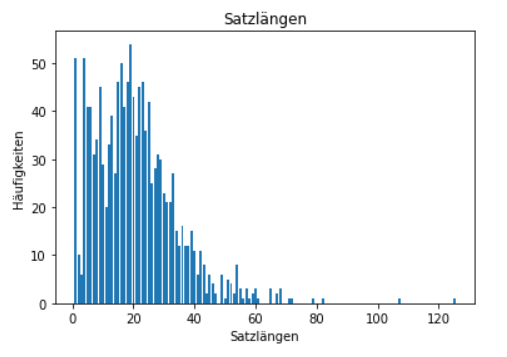
\includegraphics[scale=4]{satzlaenge.png}

\section*{Welche Links (QSLinks, OLinks) werden von welchen Präpositionen (markiert durch SPATIAL\_SIGNAL) getriggert (z.B. wie oft werden QSLinks durch die Präposition „on“ getriggert)?}

Qslink trigger:
('in', 228)
('on', 75)
('where', 68)
('at', 54)
('of', 44)
('In', 22)
('with', 15)
('along', 14)
('houses', 11)
('next to', 10)
('full of', 10)
('At', 6)
('between', 5)
('covered', 5)
('away from', 4)
('inside', 4)
('through', 4)
('around', 4)
('On', 4)
('contain', 4)
('connects', 4)
('filled', 3)
('surrounding', 3)
('from', 3)
('far from', 3)
('including', 3)
('away', 2)
('surrounded', 2)
('under', 2)
('across', 2)
('has', 2)
('on top', 2)
('outside', 2)
('over', 2)
('to', 2)
('atop', 2)
('overlooking', 2)
('apart from', 1)
('bordering', 1)
('on top of', 1)
('packed', 1)
('afar', 1)
('apart', 1)
('In front of', 1)
('behind', 1)
('inhabited', 1)
('Along', 1)
('inside of', 1)
('beside', 1)
('up to', 1)
('covering', 1)
('against', 1)
('about', 1)
('up', 1)
('surmounted', 1)
('stocked', 1)
('directly beneath', 1)
('restricted', 1)
('part         of', 1)
('Everywhere', 1)
('further', 1)
('adjacent to', 1)
('packed with', 1)
('contains', 1)
('in front of', 1)
('line', 1)
('upon', 1)
('house', 1)
('into', 1)
('Down', 1)
('for', 1)
('out of', 1)
('coiling up', 1)
('after', 1)

Olink trigger:
('on', 45)
('along', 14)
('next to', 12)
('between', 8)
('over', 7)
('down', 5)
('up', 5)
('covered', 5)
('south', 4)
('surrounded', 4)
('beneath', 4)
('below', 4)
('above', 4)
('surrounding', 3)
('of', 3)
('east of', 3)
('behind', 3)
('under', 3)
('around', 3)
('to', 3)
('overlooking', 3)
('east', 2)
('south of', 2)
('Southeast of', 2)
('in front of', 2)
('on top', 2)
('On', 2)
('Down', 2)
('atop', 2)
('in', 2)
('north', 2)
('north of', 2)
('to the left', 1)
('to SW', 1)
('on top of', 1)
('on your left', 1)
('Facing', 1)
('West of', 1)
('In front of', 1)
('Across', 1)
('neighboring', 1)
('Along', 1)
('beside', 1)
('to the west from', 1)
('up to', 1)
('alongside', 1)
('across', 1)
('surmounted', 1)
('on the right', 1)
('southwest', 1)
('adjacent to', 1)
('directly beneath', 1)
('upstream from', 1)
('overlook', 1)
('in that direction', 1)
('toward', 1)
('backwards', 1)
('west', 1)
('in the direction to', 1)
('line', 1)
('upon', 1)
('across from', 1)
('South\\xadeast of', 1)
('next door to', 1)
('facing', 1)
('northeast', 1)
('coiling up', 1) 

\section*{Welches sind die fünf häufigsten „MOTION“ Verben (und wie oft kommen diese vor)?}

('bike', 68)	\\
('go', 38)		\\
('visit', 35)  \\
('drive', 32)  \\
('leave', 32)  \\

\section*{Visualisierung}
\subsection*{Bicycle.xml}
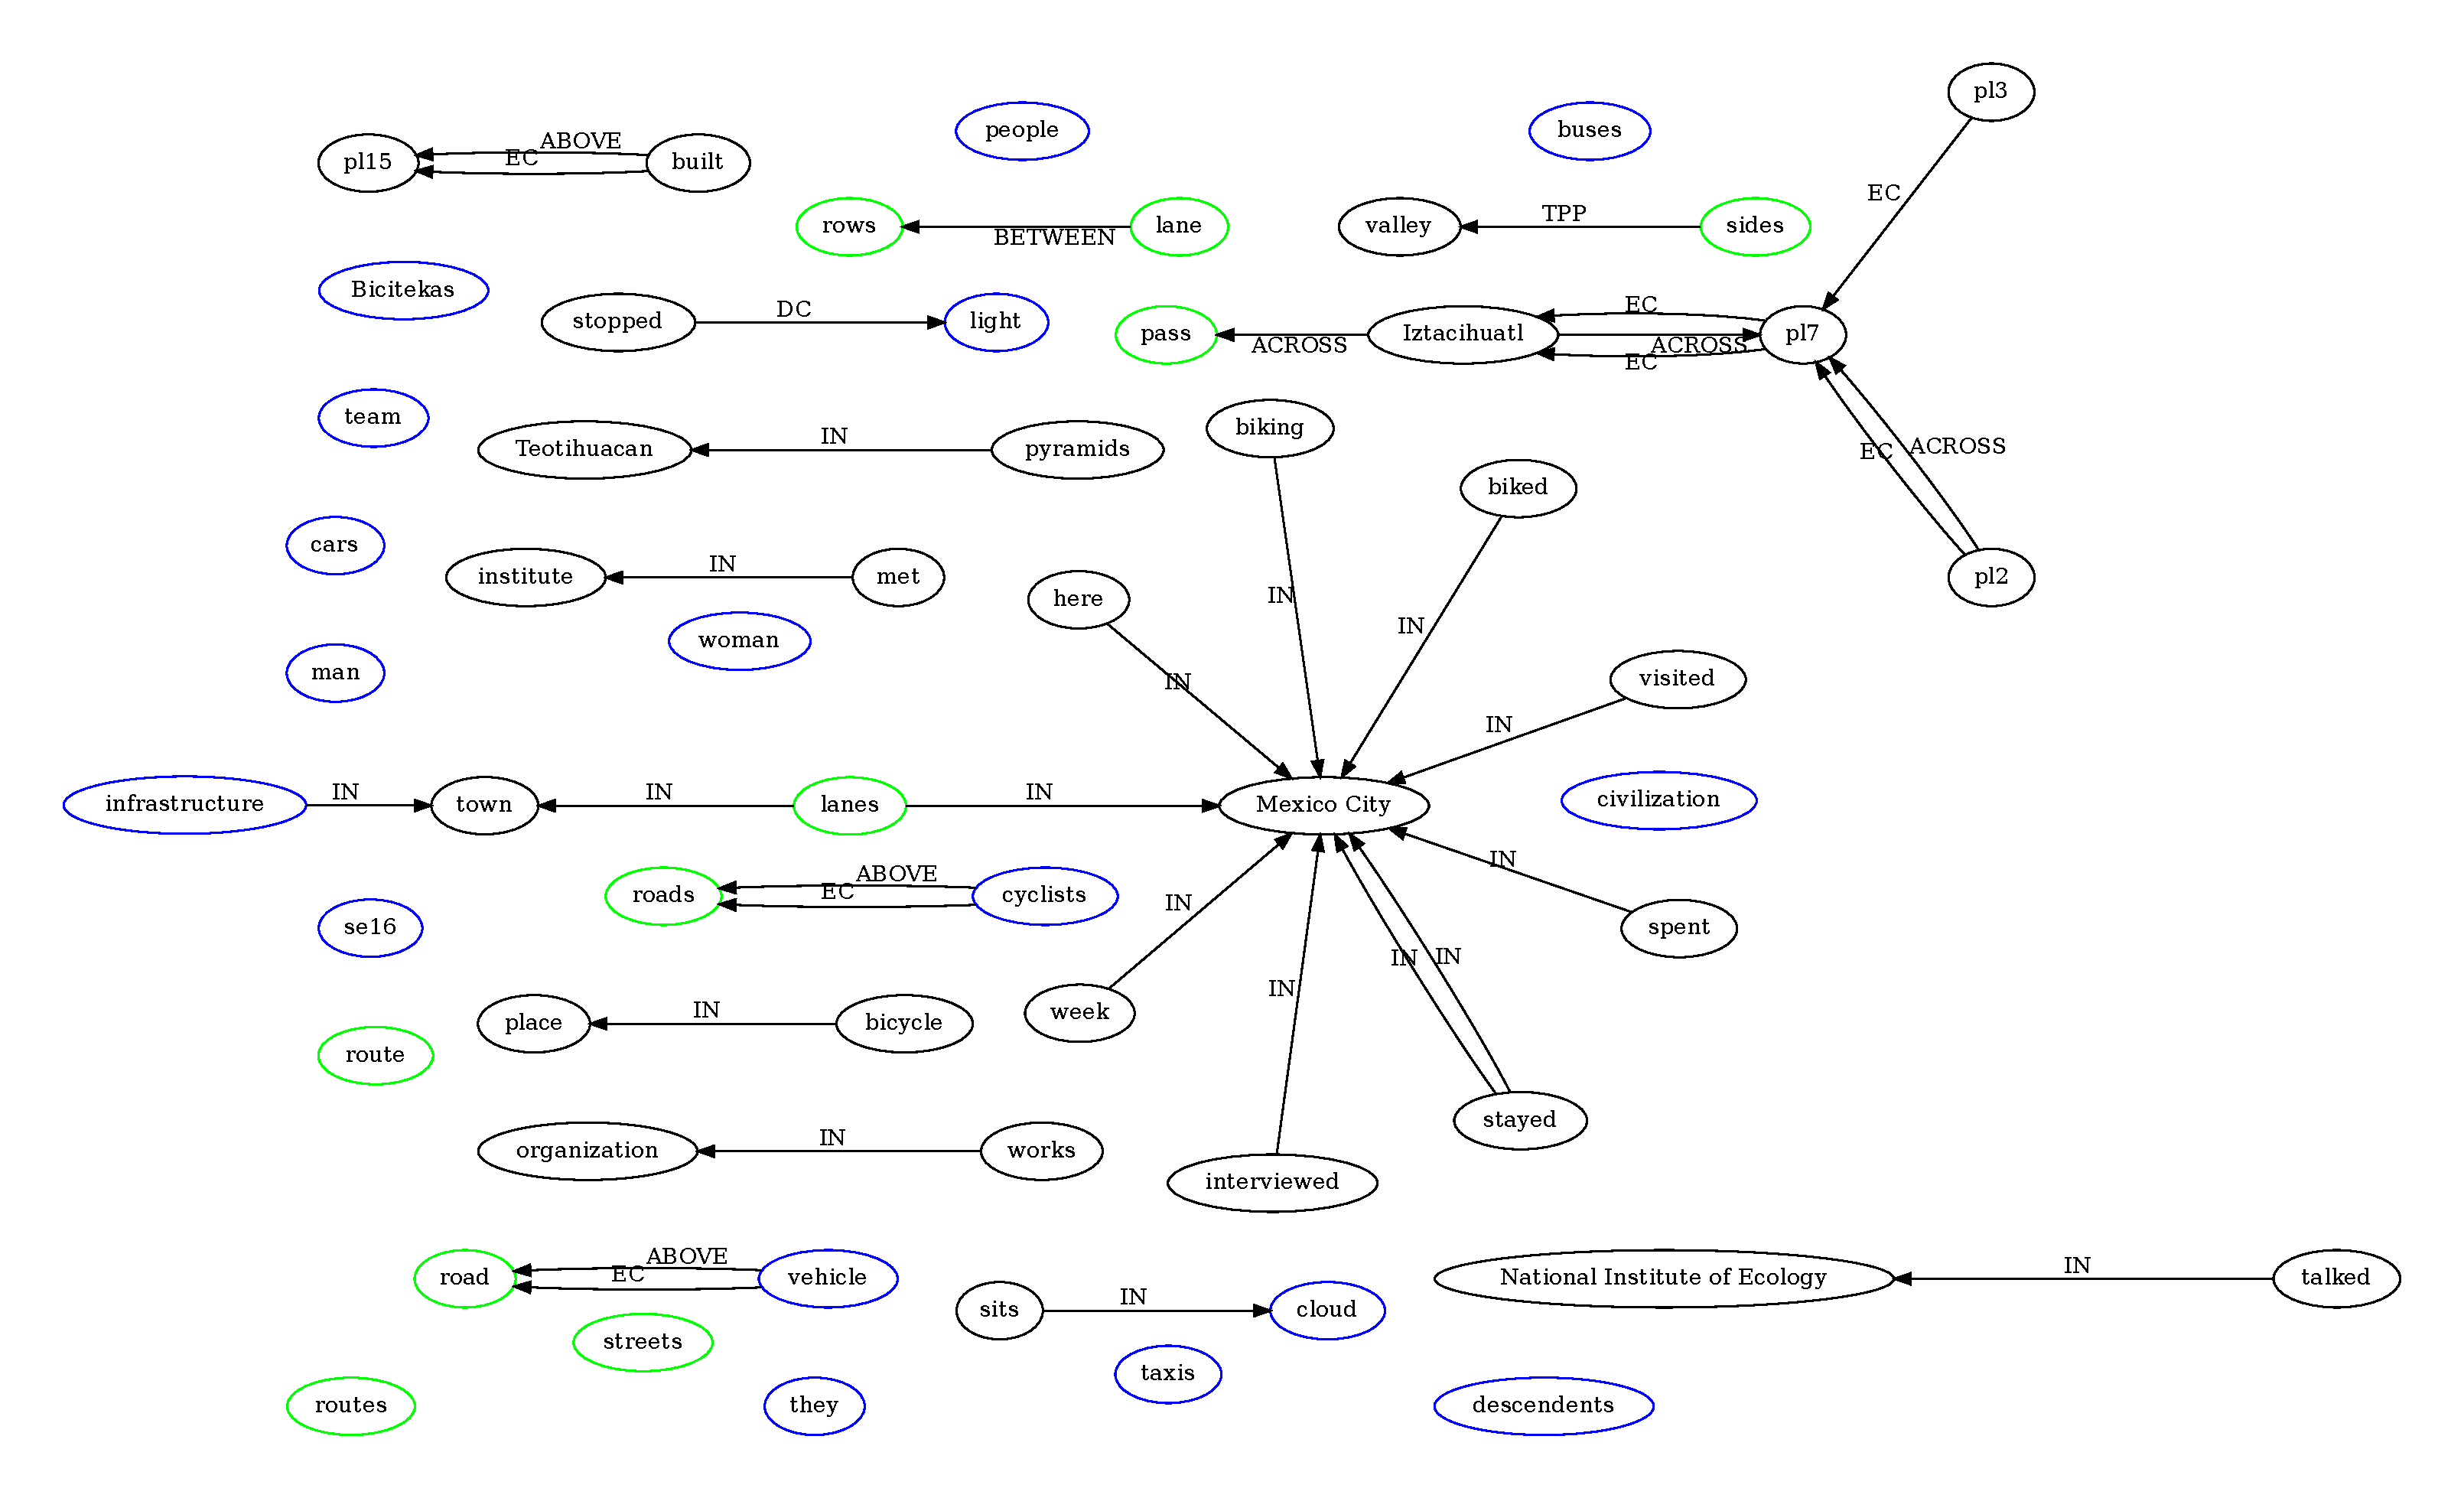
\includegraphics[scale=0.35]{../bicycle.gv.pdf}
\subsection*{Museum.xml}
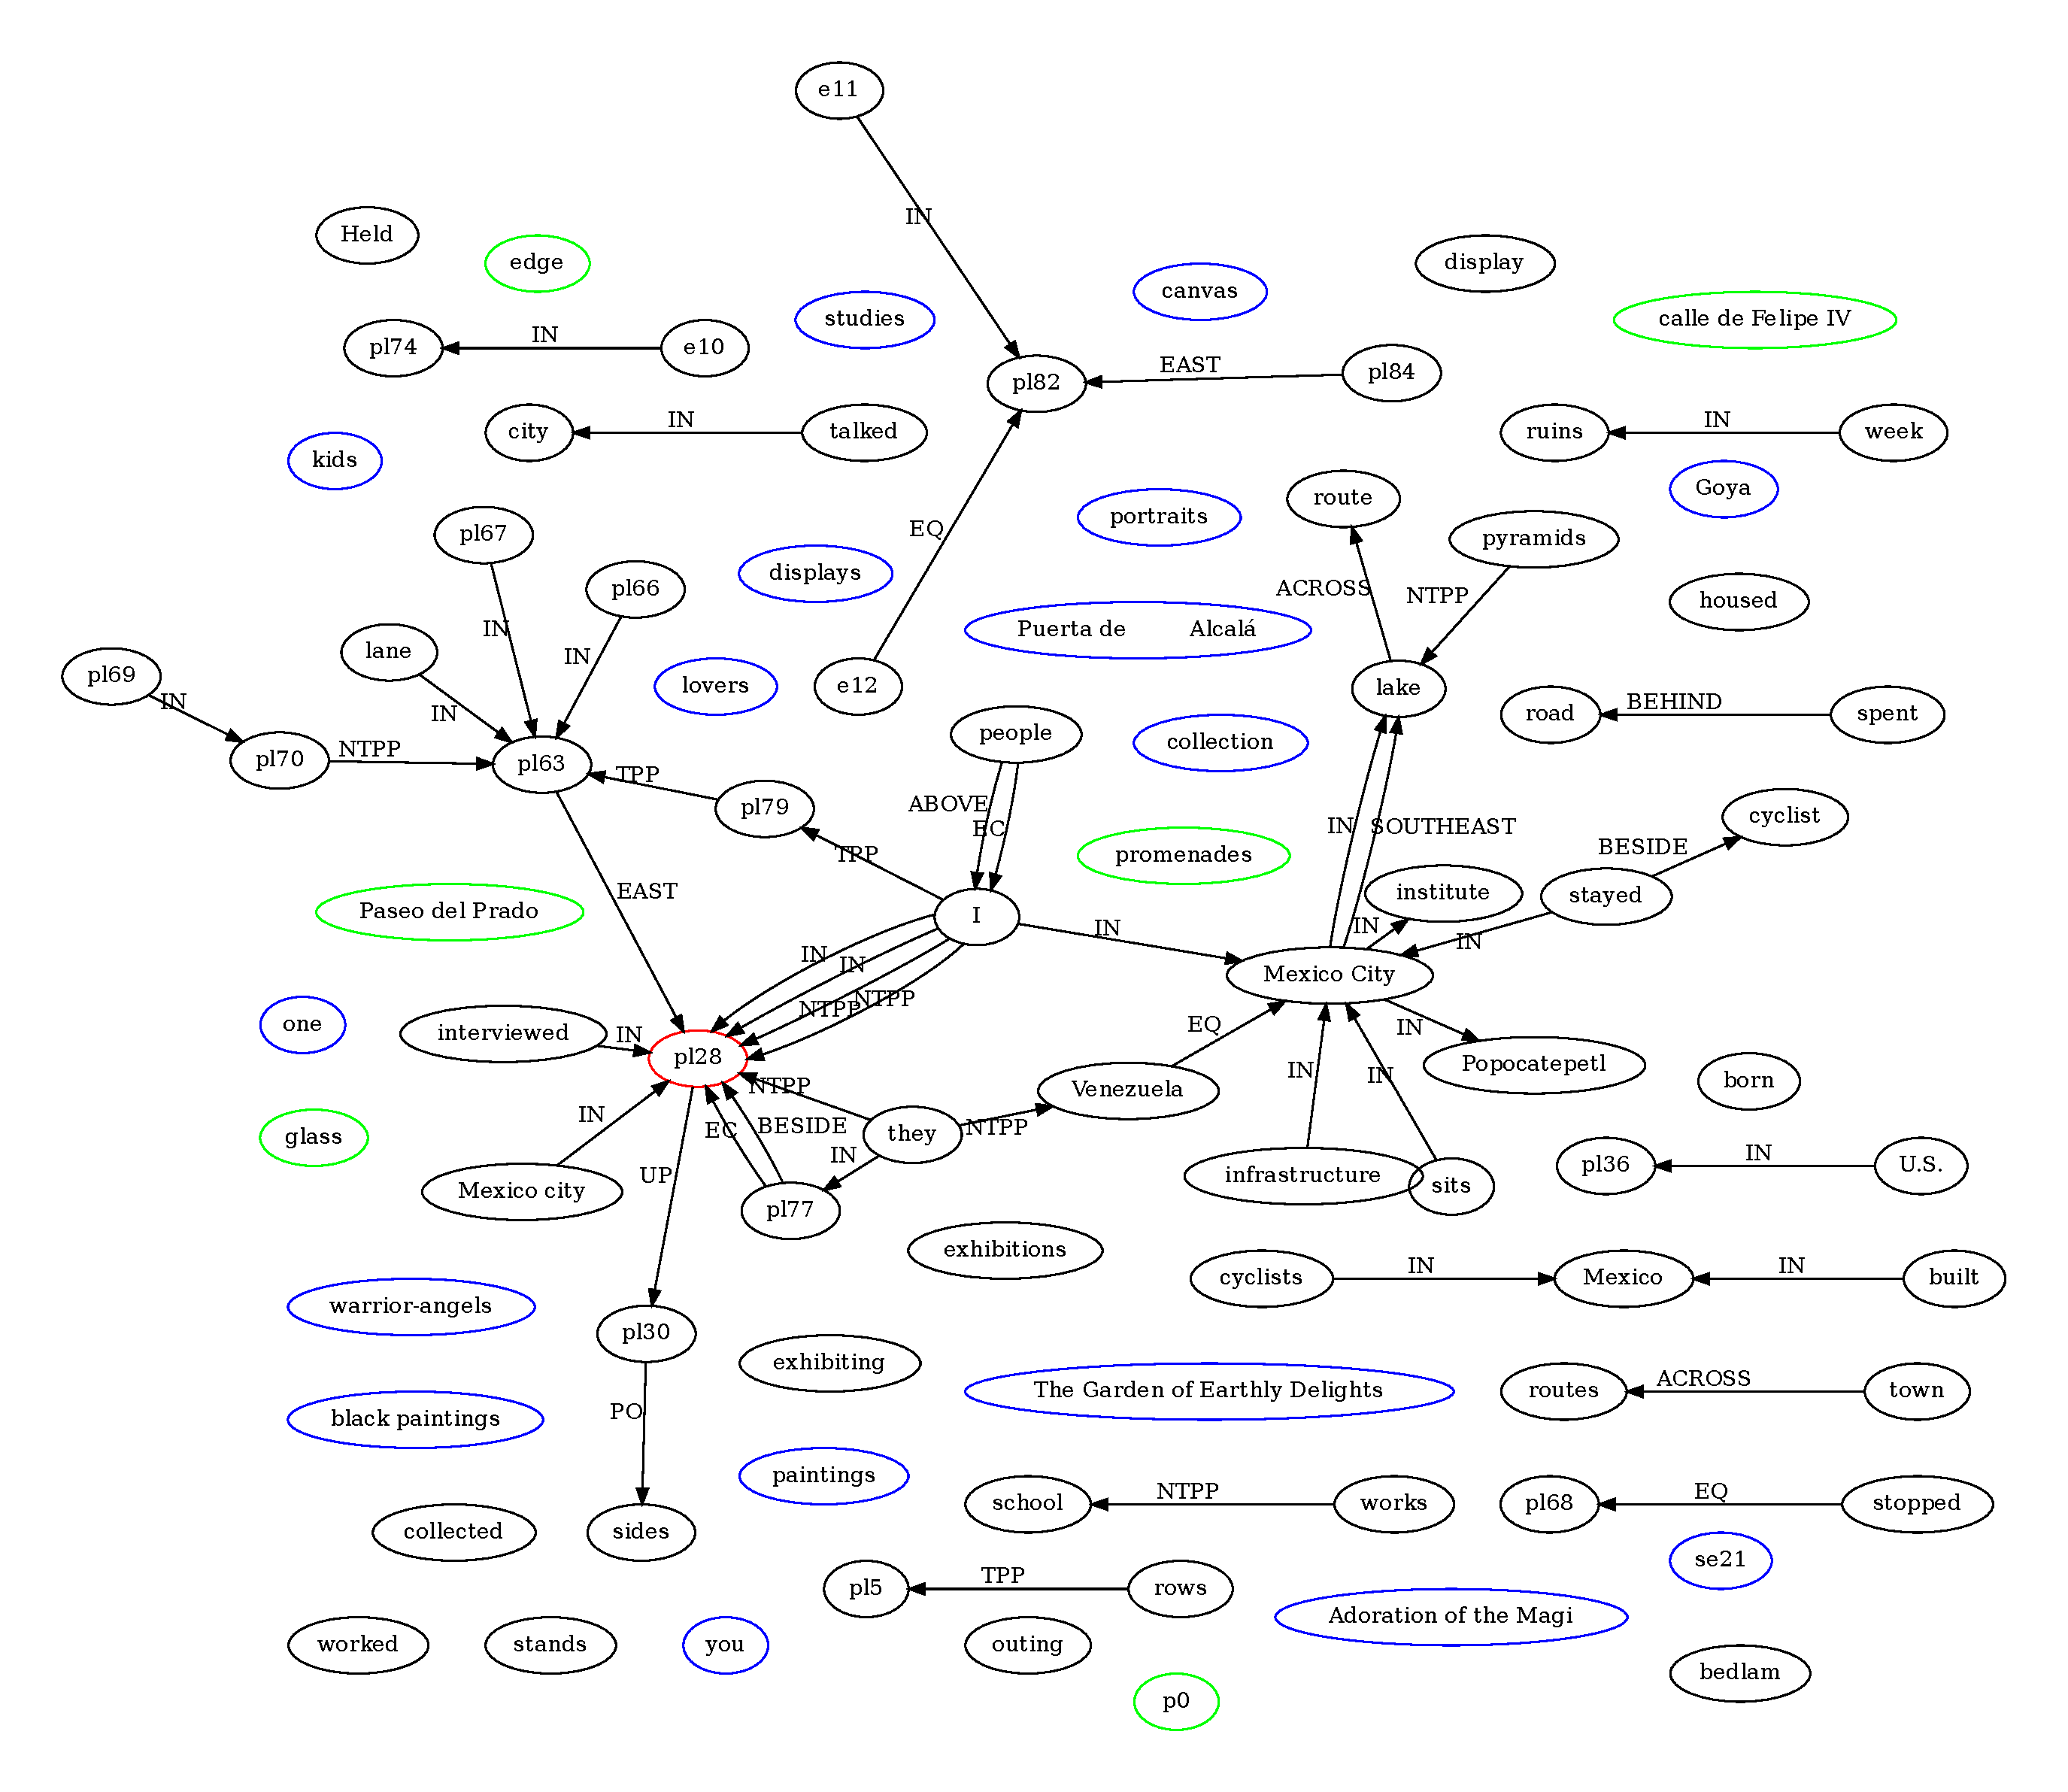
\includegraphics[scale=0.2]{../museum.gv.pdf}
 
\end{document}